\begin{opgave}{Diatomare molekyler}{1}
\begin{figure}[h]
\center
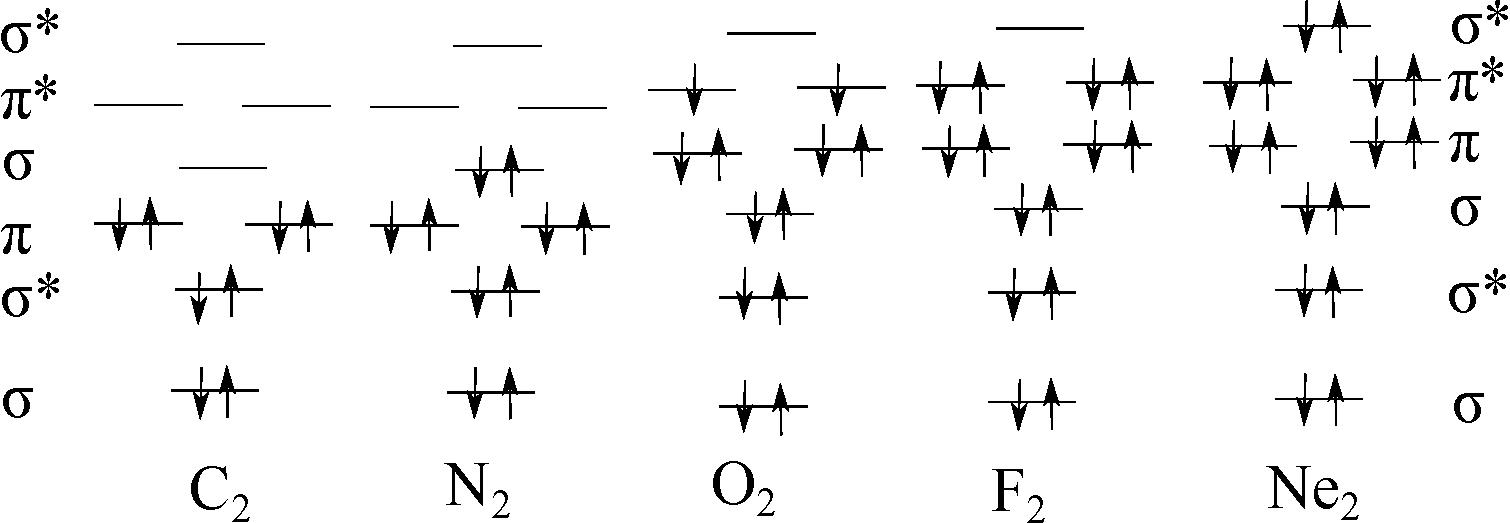
\includegraphics[width = \textwidth]{Atom-ogMolekylefysik/billeder/diatomar.pdf}
\caption{Molekyleorbitaldiagrammer of diatomare molekyler.}
\label{opg:diatomar}
\end{figure}
\opg Diatomare molekyler lettere end N$_2$ har samme struktur af orbitaler som N$_2$. De tungere har samme struktur som O$_2$.
\opg Bindingsorden er antallet af fyldte bindende orbitaler minus antallet af fyldte antibindende orbitaler, så:
\begin{tabular}{c|c c c c c}
&C$_2$&N$_2$&O$_2$&F$_2$&Ne$_2$\\\hline
$b$&2&3&2&1&0
\end{tabular}
\opg N$_2$ vil være det mest ustabile, da det har den laveste bindingsorden, og ganske rigtigt Findes Ne$_2$ ikke. C$_2$ forekommer hellerikke, men det er fordi kulstof kan danne andre strukturer så som diamant og grafit, der er mere stabile.
\opg Kun O$_2$ har uparrede elektroner, så det er det eneste af molekylerne der er magnetisk.
\end{opgave}
\begin{opgave}{Vand}{2}
\opg Brintmolekylet har den bindende og den anti bindende $\sigma$ orbital.
\begin{figure}[h]
\center
\includegraphics[width = \textwidth]{Atom-ogMolekylefysik/billeder/tilstande1.pdf}
\end{figure}
\opg
Det frie ilt har $1s$, $2s$ og $2p$ orbitalerne, men $1s$ ligger meget lavere end de andre og indgår ikke i bindingen.
\begin{figure}[h]
\center
\includegraphics[width = \textwidth]{Atom-ogMolekylefysik/billeder/tilstande2.pdf}
\end{figure}
\opg
Lægges bindingsaksen for H$_2$ langs $y$-aksen og føres ind imod O-atomet langs $z$-aksen. Så vil orbitalerne overlappe hvis de kan have fælles fortegn i hele kontaktområdet. Det betyder at $p_x$ ikke overlapper med nogle da den kan en knudeflade i $yz$-planen, som ingen andre orbitaler har. $p_y$ overlapper med $\sigma^*$. Derudover overlapper $\sigma$ med både $s$ og $p_z$.
\opg For at opstille molekyleorbitaldiagrammet ser man på tabel 4.1 for energien af O orbitalerne. H$_2$ orbitalerne er en slat lavere end $1s$ for brintatomet, for $\sigma$ og højere for $\sigma^*$.
$p_x$ forbliver uændret, da den ikke har noget overlap. 
$\sigma^*$ og $p_y$ viser sig at give en stor opsplitning. Disse orbitaler kaldes af grunde vi desværre ikke var i stand til at dække $1b_2$ og $2b_2$. De spøjse navne stammer fra en måde at kategorisere molekylers symmetri, baseret på gruppeteori.
De sidste tre orbitaler har en hævet, en imidten og en lav. disse kaldes $4a_1$, $3a_1$ og $2a_1$. På figuren kalds den uændrede $p_x$-orbital også for $b_1$

Det vigtige er at vide hvilke orbitaler der interagerer og hvordan det fører til opsplitning, graden af opsplitning er ikke super essentiel, da det ikke er muligt at udregne med de værktøjer vi har præsenteret her.

Elektroner indsættes efter Aufbau princippet nedefra.
\begin{figure}[h]
\center
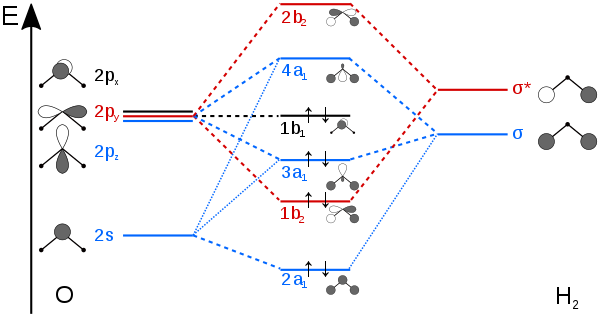
\includegraphics[width = \textwidth]{Atom-ogMolekylefysik/billeder/H2O-MO-Diagram-wiki.png}
\caption{Molekyleorbitaldiagrammet for vand.}
\end{figure}
\opg At afgøre om orbitaler er bindende, antibindende eller ikke bindende er ikke helt så simpelt som for homoatomare diatomiske molekyler, men det gøres lettest ved at sammenligne hver orbital med de tilsvarende i det ubundne molekyle. Det giver at de to nederste to orbitaler, $2a_1$ og $1b_2$, er bindende, $3a_1$ og $1b_1$ er ikke bindende og $4a_1$ og $2b_2$ er antibindende.
\opg Der er to fyldte bindende orbitaler og to ikke bindende, så bindingsordenen er 2, svarende til to enkeltbindinger.
\end{opgave}
\begin{opgave}{Benzen}{3}
\opg Index viser hvor langt rundt langs ringen det tilhørende atom er, så $p_7$ svarer til $p_1$. 
\opg $p$-orbitalerne giver allerede en knudeflade i ringens plan. Ønskes så få som muligt vil alle $p$ orbitalerne med samme fortegn give ingen nye knudeflader.
$$
1\pi = \sum_{i=1}^6 p_i = p_1+p_2+p_3+p_4+p_5+p_6
$$
\opg
Gives de alternerende forgen kommer der tre knudeflader imellem alle atomerne.
$$
6\pi = \sum_{i=1}^3 (p_{2i}-p_{2i+1})=p_1+p_2+p_3-p_4+p_5-p_6
$$
\begin{figure}
\center
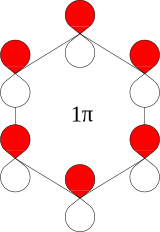
\includegraphics[width = 0.45\textwidth]{Atom-ogMolekylefysik/billeder/benzen1}
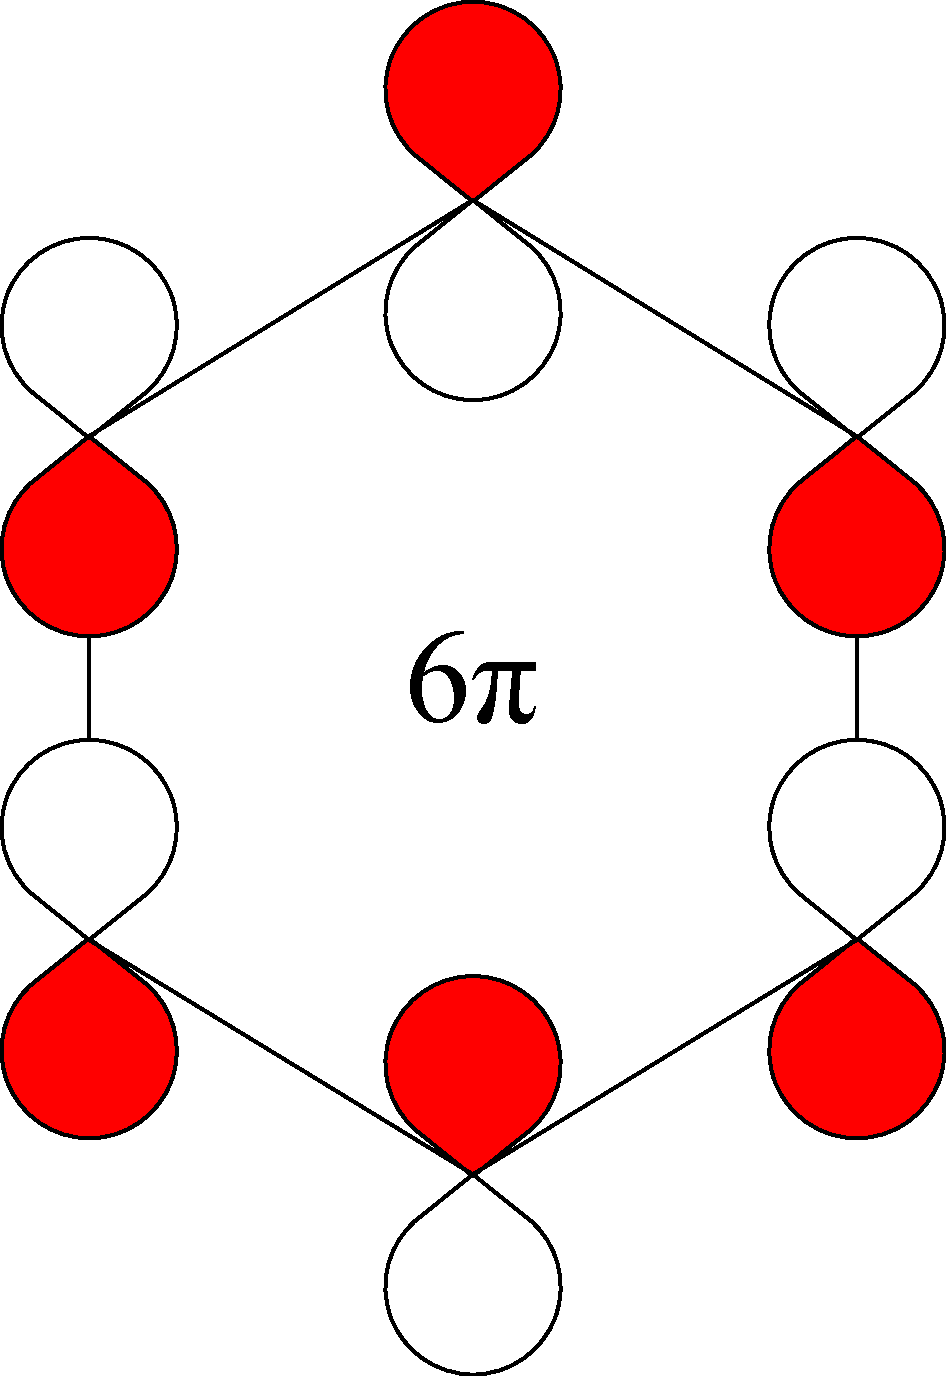
\includegraphics[width = 0.45\textwidth]{Atom-ogMolekylefysik/billeder/benzen6}
\caption{De to tilstande $1\pi$(til venstre) og $6\pi$(til højre).}
\end{figure}
\opg For $1\pi$ er sum notation et godt værktøj.
\begin{align*}
\op H 1\pi &= \op H \sum_{i=1}^6\\
&= \sum_{i=1}^6 \op Hp_i\\
&= \sum_{i=1}^6 (\alpha p_i+\beta p_{i-1}+\beta p_{i+1})\\
&= \sum_{i=1}^6 \alpha p_i+\sum_{i=1}^6\beta p_{i-1}+\sum_{i=1}^6\beta p_{i+1}\\
&= \alpha \sum_{i=1}^6 p_i+2\beta \sum_{i=1}^6 p_i\\
&= (\alpha +2\beta)1\pi
\end{align*}
Så energien er:
$$
E=\alpha + 2\beta
$$
For $6\pi$ har vi:
\begin{align*}
\op H 6\pi &= \op H \sum_{i=1}^3 (p_{2i}-p_{2i+1})\\
&=\sum_{i=1}^3 (\alpha p_{2i}+\beta p_{2i-1}+\beta p_{2i+1}-\alpha p_{2i+1}-\beta_{2i}-\beta p_{2i+2})\\
&= \alpha \sum_{i=1}^3 (p_{2i}-p_{2i+1})+\beta\sum_{i=1}^3(p_{2i-1}+p_{2i+1}-p_{2i}-p_{2i+2})\\
&=\alpha 6\pi+\beta\sum_{i=1}^3(p_{2i-1}-p_{2i})+(p_{2i+1}-p_{2i+2})\\
&=\alpha6\pi-\beta\left(\sum_{i=1}^3(p_{2i}-p_{2i-1})+\sum_{i=1}^3(p_{2i+2}-p_{2i+1}\right)\\
&= (\alpha-2\beta)6\pi
\end{align*}
Så energien er:
$$
\alpha-2\beta
$$
\opg $1\pi$ skal have den mindste energi, så $\beta$ må være negativ.
\opg
Der er fejl i denne opgave, første $2\pi$ skulle have været:
$$
2\pi = \frac{1}{2\sqrt{3}}\left(2p_1+p_2-p_3-2p_4-p_5+p_6\right)
$$
Desuden skulle den anden  $2\pi$ have været $4\pi$ \& anden $3\pi$ have været $5\pi$.
\begin{figure}[h]
\center
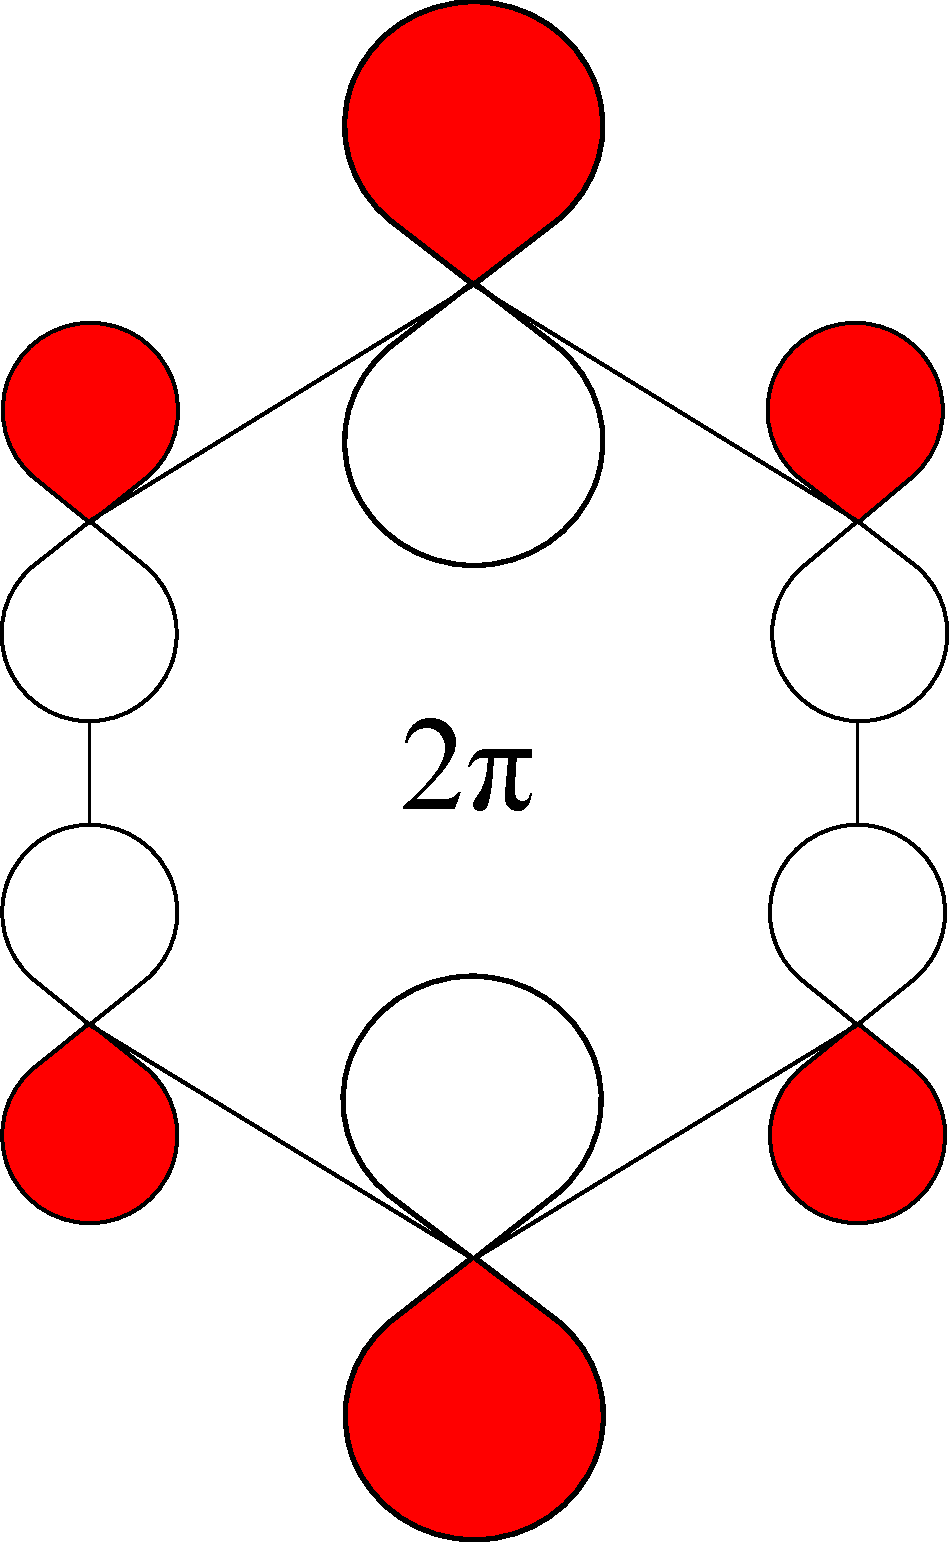
\includegraphics[width = 0.35\textwidth]{Atom-ogMolekylefysik/billeder/benzen2.pdf}
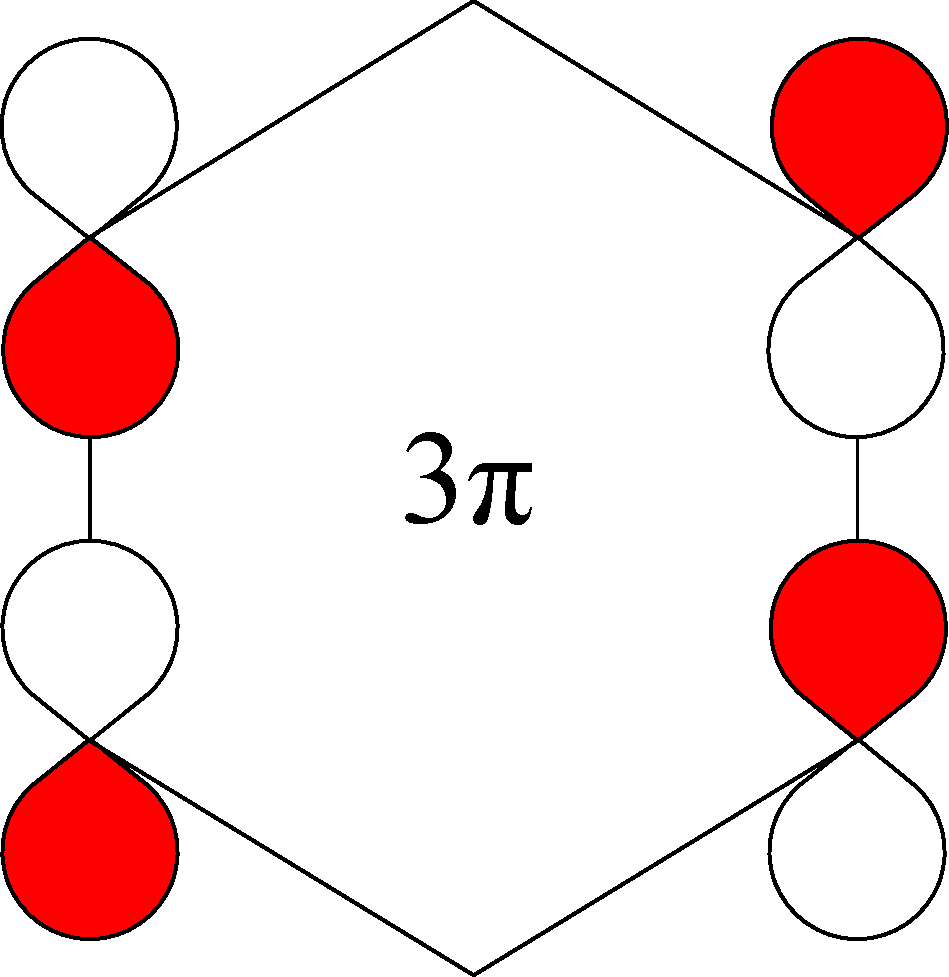
\includegraphics[width = 0.35\textwidth]{Atom-ogMolekylefysik/billeder/benzen3.pdf}
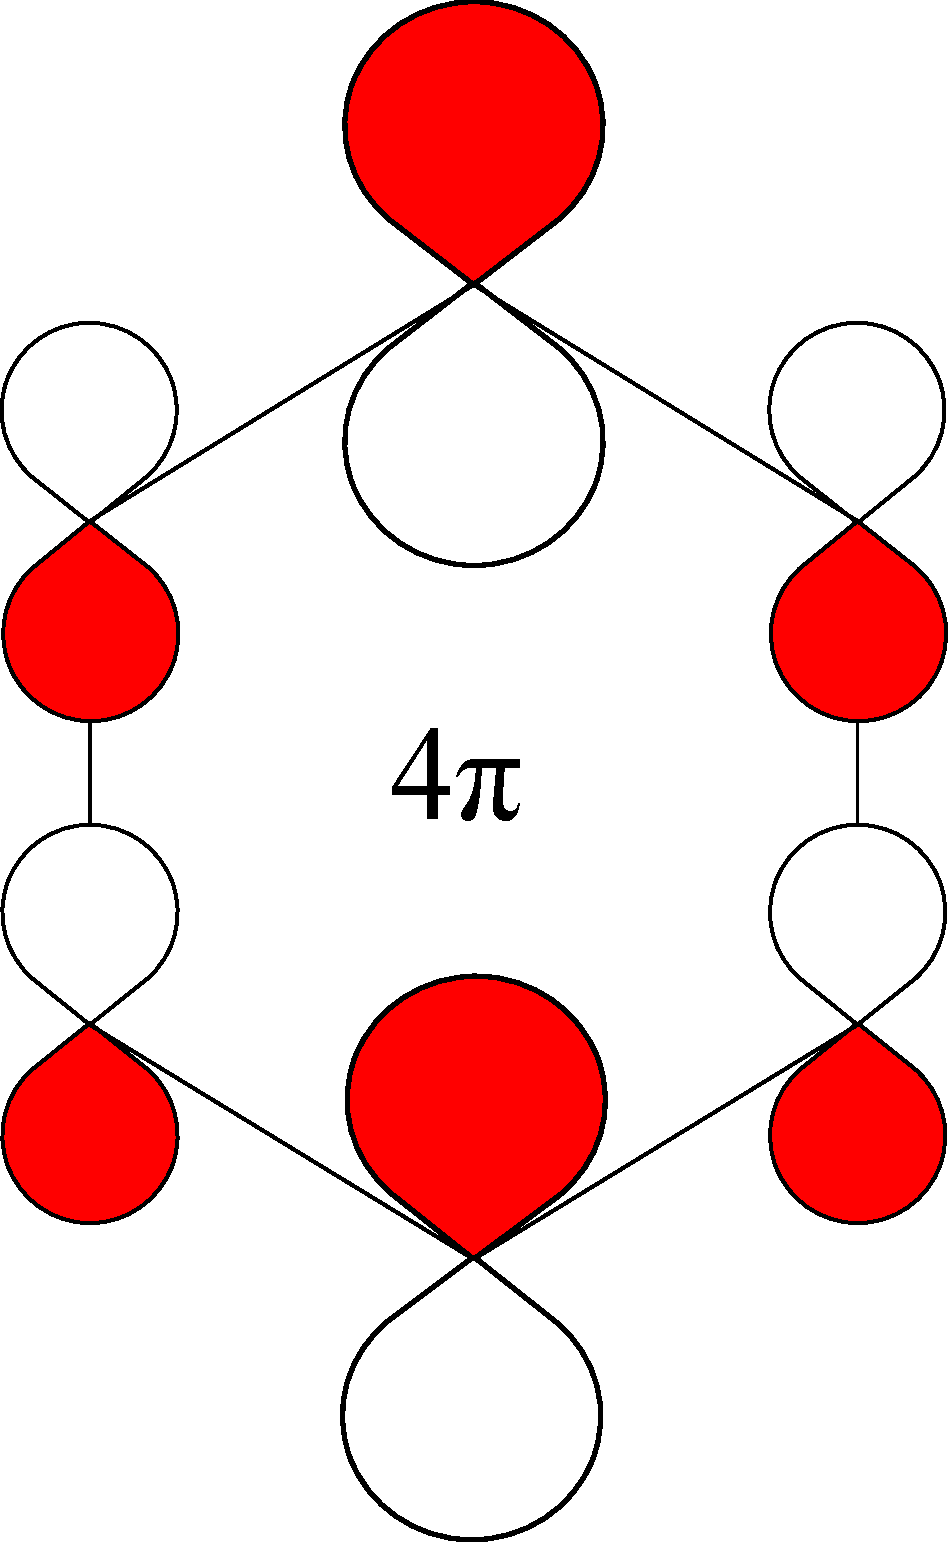
\includegraphics[width = 0.35\textwidth]{Atom-ogMolekylefysik/billeder/benzen4.pdf}
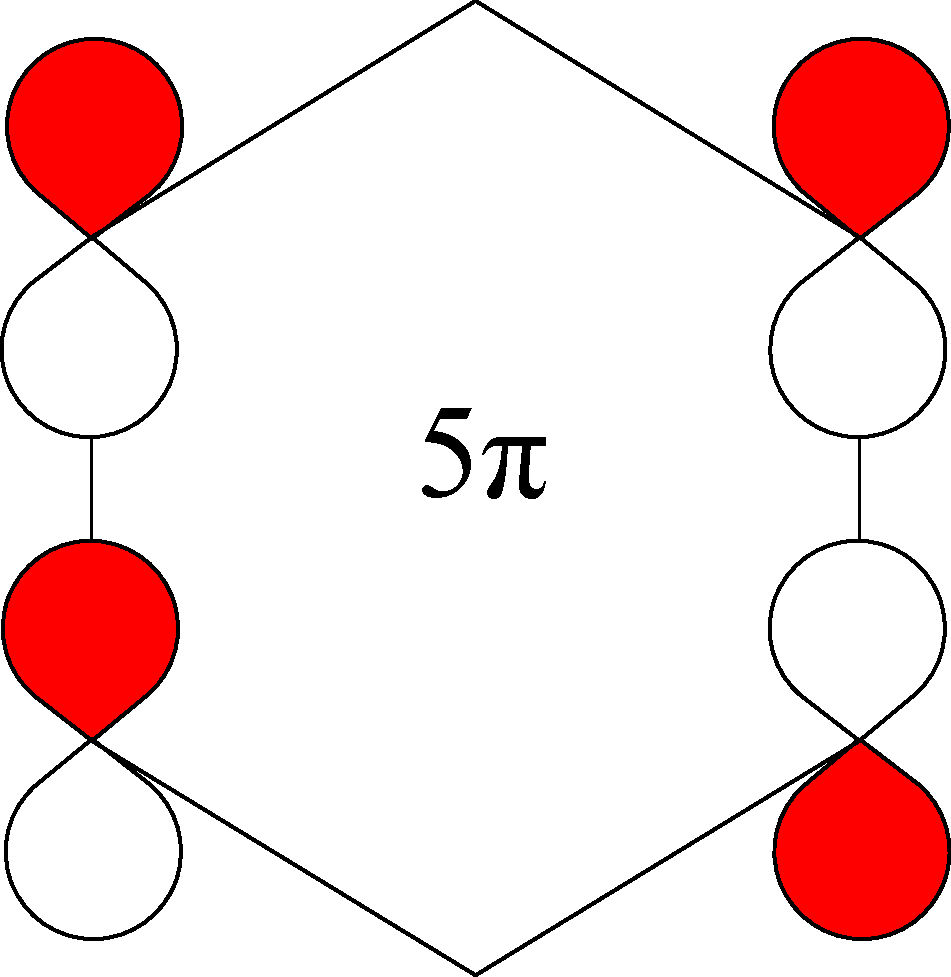
\includegraphics[width = 0.35\textwidth]{Atom-ogMolekylefysik/billeder/benzen5.pdf}
\caption{Skitser af de fire mellemste $\pi$-orbitaler}
\end{figure}
\opg
For at opstille molekyleorbitaldiagrammet er det nødvendigt at kende de sidste bølgefunktioners energi. Energien findes ved at anvende Hamiltonoperatoren på de fire tilstande.
\begin{align*}
\op H 2\pi &= \op H \frac{1}{2\sqrt{3}}(2p_1+p_2-p_3-2p_4-p_5+p_6)\\
&= \frac{1}{2\sqrt{3}}(\alpha(2p_1+p_2-p_3-2p_4-p_5+p_6)+\beta(2p_6+p_1-p_2-2p_3-p_4+p_5)+\beta(2p_2+p_3-p_4-2p_5-p_6+p_1))\\
&=\frac{1}{2\sqrt{3}}(\alpha(2p_1+p_2-p_3-2p_4-p_5+p_6)+\beta(2p_1+p_2-p_3-2p_4-p_5+p_6)\\
&=(\alpha+\beta)2\pi\\
\op H 3\pi &= \op H\frac{1}{2} (2p_2+p_3-p_5-p_6)\\
&= \frac{1}{2}(\alpha((2p_2+p_3-p_5-p_6)+\beta((2p_1+p_2-p_4-p_5)+\beta((2p_3+p_4-p_6-p_1))\\
&=\frac{1}{2}(\alpha(2p_2+p_3-p_5-p_6)+\beta(2p_2+p_3-p_5-p_6)\\
&=(\alpha+\beta)3\pi\\
\op H 4\pi &= \op H \frac{1}{2\sqrt{3}}(2p_1-p_2-p_3+2p_4-p_5-p_6)\\
&=\frac{1}{2\sqrt{3}}(\alpha(2p_1-p_2-p_3+2p_4-p_5-p_6)+\beta(2p_6-p_1-p_2+2p_3-p_4-p_5)+\beta(2p_2-p_3-p_4+2p_5-p_6-p_1))\\
&=\frac{1}{2\sqrt{3}}(\alpha(2p_1-p_2-p_3+2p_4-p_5-p_6)+\beta(-2p_1+p_2+p_3-2p_4+p_5+p_6))\\
&=(\alpha-\beta)4\pi\\
\op H 5\pi &= \op H\frac{1}{2}(p_2-p_3+p_5-p_6)\\
&= \frac{1}{2}(\alpha(p_2-p_3+p_5-p_6)+\beta(p_1-p_2+p_4-p_5)\beta(p_3-p_4+p_6-p_1))\\
&= \frac{1}{2}(\alpha(p_2-p_3+p_5-p_6)+\beta(-p_1+p_2-p_5+p_6))\\
&=(\alpha-\beta)5\pi
\end{align*}
Nu hvor vi kender energien kan vi opstille et molekyleorbitaldiagram.
\begin{figure}[h]
\center
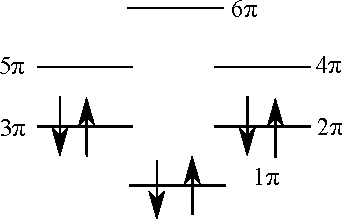
\includegraphics[width = \textwidth]{Atom-ogMolekylefysik/billeder/benzenMO.pdf}
\caption{Molekyleorbitaldiagram for benzens $\pi$ system.}
\end{figure}
\end{opgave}
\begin{figure}[t]
	\centering
	%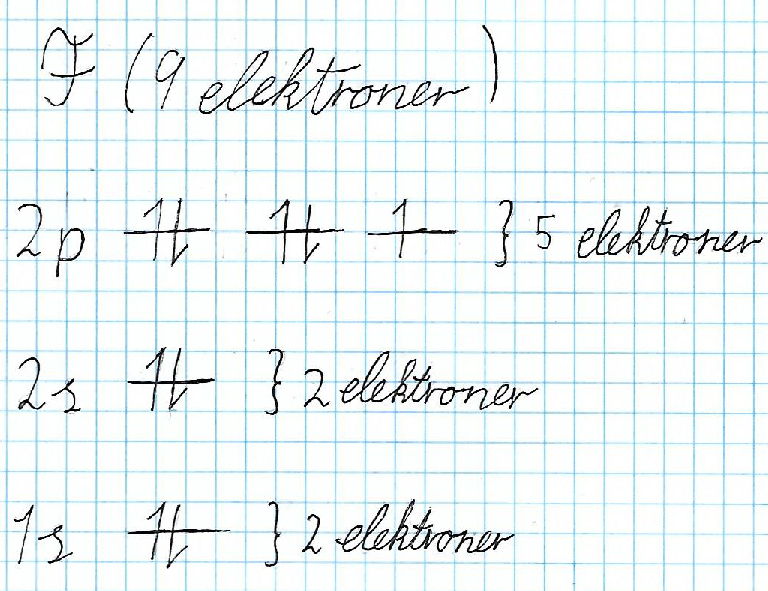
\includegraphics[width=\columnwidth]{Atom-ogMolekylefysik/billeder/F.pdf}
	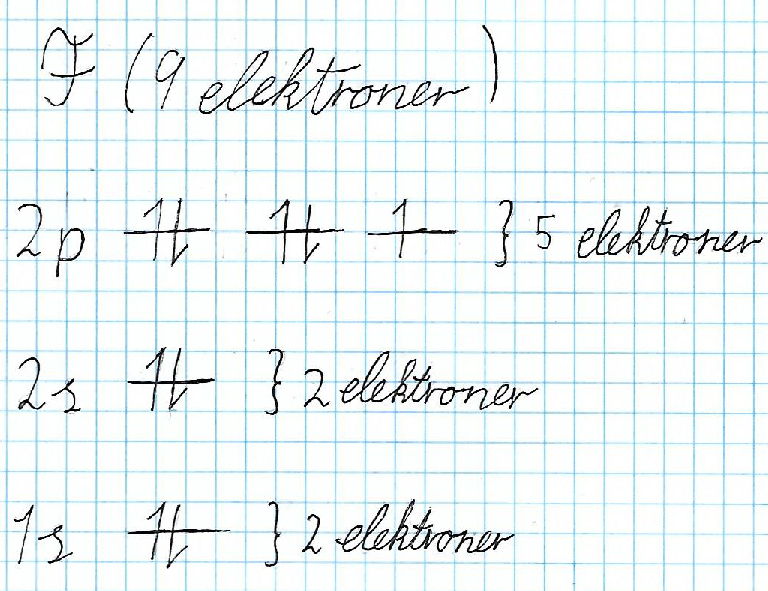
\includegraphics[width=\columnwidth]{Atom-ogMolekylefysik/billeder/F.pdf}
	\caption{Elektronstrukturen for F.} \label{fig:F}
\end{figure}
\begin{figure}[t]
	\centering
	%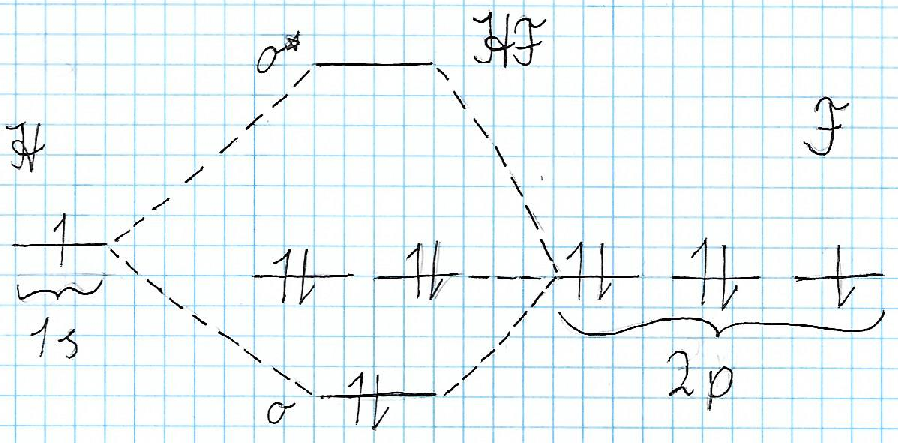
\includegraphics[width=\columnwidth]{Atom-ogMolekylefysik/billeder/HF.pdf
	\includegraphics[width=\columnwidth]{Atom-ogMolekylefysik/billeder/HF.pdf}
	\caption{Elektronstrukturen for HF, hvor de to midterste er ikke-bindende $p$-orbitaler. Bemærk at $\sigma^*$-orbitalen er tom, samt at alle elektronerne befinder sig i en tilstand med samme eller lavere energi end før.} \label{fig:HF}
\end{figure}
\begin{figure}[t]
	\centering
	%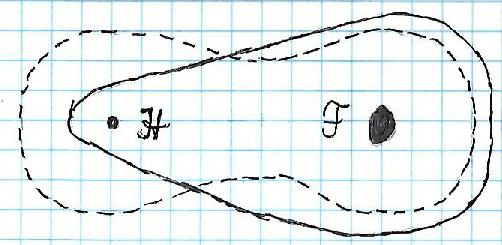
\includegraphics[width=\columnwidth]{Atom-ogMolekylefysik/billeder/HF_orbit.pdf}
	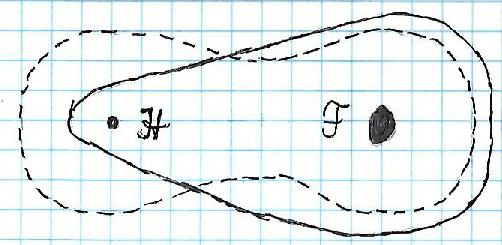
\includegraphics[width=.9\columnwidth]{Atom-ogMolekylefysik/billeder/HF_orbit.pdf}
	\caption{Skitse den bindende $sigma$-orbital for HF, hvor den stiplede linje indikerer hvordan den ville se ud, hvis man ikke tager højde for forskellene mellem H og F, mens den fuldtoptrukne tager denne forskel i betragtning.} \label{fig:HF_orbit}
\end{figure}
\begin{opgave}{Halogener og hydrogenbindinger}{3}
\opg Se figur \ref{fig:F}
\opg Fra forgående spørgsmål ses det at flour mangler 1 elektron for at have sin yderste $p$-orbital fuld, og dermed opnå den stabile tilstand af en fuld yderste $s$- og $p$-orbital, hvilket gælder for alle halogenerne.
\opg De to $s$-orbitaler deltager ikke i bindingen, hvorfor de ikke tegnes. I figur \ref{fig:HF} ses det at elektronerne er i en lavere energitilstand, hvis de to atomer bindes til hinanden, end hvis de holder sig hver for sig.
\opg Bindingen er en $\sigma$-binding, da den er mellem en $s$- og en $p$-orbital.
\opg Hydrogen findes ofte som ${}^1$H, hvilket vil sige at det består af en proton og en elektron, men ingen neutroner. En proton er stabil som sig selv, mens flour meget gerne vil have en elektron til at fylde sin sidste $p$-orbital. Flour trækker derfor meget mere i $\sigma$-orbitalen end hydrogen, hvilket forskyder orbitalen mod flour, som illustreret i figur \ref{fig:HF_orbit}.
\opg Eftersom H i gennemsnit "mangler" sine elektroner, er det en "åben proton". Der er ikke noget, der skærmer den i retningen væk fra flour, hvorfor den tiltrækker alt hvad der er negativt. Det gælder både det flouratom, den er bundet til, hvorfor bindingslængden er ekstremt kort, men det gælder også flouratomer i andre HF-molekyler. Derfor tiltrækker den negative del af et HF-molekyle den positive del af et andet HF-molekyle, hvilket er hvad der kaldes en hydrogenbinding. I nogle tilfælde er hydrogenbindingen faktisk så stærk, at orbitalerne fra to tilstødende molekyler begynder at overlappe, hvilket gør at båndet får kovalent karakter, fremfor at opføre sig rent som en intermolekylær kraft.
\opg Tages chlor som eksempel, så er $Cl$ grundstof nummer 17, hvilket betyder at orbitalerne $1s$, $s2$, $2p$ og $3s$ er fyldte, mens det er $3p$-orbitalen, der mangler en elektron, for at være fuld. Det betyder at der er markant flere elektroner omkring chlor, og elektroner frastøder hinanden, hvorfor chlor ikke kan trække så meget i det bindende elektronpar. Man siger at kernen er skærmet og har en mindre effektiv kerneladning. Chloratomet kan derfor ikke trække elektronparet ligeså tæt på sig som flour kan, og det befinder sig derfor tættere på H. Derudover kommer H ikke så tæt på Cl, som det kan komme på F, hvorfor ladningsforskydningen eller dipolmomentet ikke er stort nok til at danne hydrogenbindinger. Da både brom og iod er større end chlor gælder dette også for dem. Det er netop det at $\mathrm{HF}(aq)$ er så svært at styrre, og det forklarer også hvorfor de andre hydrogenhalider er stærkere syrer end flussyre.
\end{opgave}